\section{Numerical-Domain Diagnostics}
\setcounter{equation}{0}\setcounter{table}{0}\setcounter{figure}{0}
\label{app:numerical-domain-diagnostics}

\label{app:domain-choice}

The primary computational domain is \(A_0=[-1,3]\), evaluated on 41 equally spaced candidate values with step size \(h=0.1\). 
Using the same domain for all sample sizes, quantiles, instrument-relevance settings, and estimators makes the accepted-set measures directly comparable across the simulation design.

The interval also contains the true structural quantile effects for all five investigated quantiles. Under the data-generating process,
\[
\alpha_0(\tau)=1+\Phi^{-1}(\tau),
\]
so the true effects are approximately \(-0.282\), \(0.326\), \(1.000\), \(1.674\), and \(2.282\) for \(\tau=0.10,0.25,0.50,0.75,\) and \(0.90\), respectively. All five structural truths lie strictly inside \(A_0\); using their unrounded values, the minimum distance to either endpoint is approximately \(0.718\). The interval should therefore be understood as a common numerical search domain, not as an assumed theoretical parameter space.

A finite search domain can nevertheless become restrictive when instruments are weak and many candidate values are accepted. For this reason, a separate sensitivity diagnostic expands the search range from \(A_0=[-1,3]\) to \(A_1=[-3,5]\) and then to \(A_2=[-5,7]\). Under strong instrument relevance, expanding the domain adds little accepted measure, indicating that the observed accepted components are well localized within the investigated ranges. At intermediate relevance, the wider domains contain additional accepted values in some profiles. Under the weakest relevance setting, the accepted measure continues to increase as the domain is expanded and does not stabilize within \(A_2\).

These results clarify the interpretation of the main accepted-set measure. A value close to four in \(A_0\) means that almost the entire four-unit primary domain is accepted; it does not mean that the unrestricted confidence region has length four. Similarly, continued acceptance in the wider domains indicates poor numerical localization over the ranges examined, but it does not by itself establish that the theoretical confidence region is globally unbounded or that identification completely fails.

Table~\ref{tab:appendix-grid-measures} retains the key frozen domain-measure comparisons; Figure~\ref{fig:grid-domain} summarizes the expansion pattern.


The main diagnostic contains one singular-design error: replication 35, $\tau=0.90$, $\kappa=0.10$, DML-IVQR, candidate $a=-2.1$ in Stage 1. Stage 2 adds no new evaluation errors. Incomplete profiles receive missing aggregate measures; the affected expanded-domain cell therefore uses 99 usable replications, while other displayed cells use 100. Tables~\ref{tab:appendix-grid-added}--\ref{tab:appendix-grid-status} retain incremental measures, boundary frequencies, profile counts, and localization diagnostics. In these tables, Med. and Mean denote replication medians and means; $R$ is the intended replication count, Succ. counts complete profiles, Fail counts incomplete profiles, and Stage 1/2 counts newly recorded evaluation errors. Boundary frequencies refer to acceptance of either endpoint; full-grid frequencies require acceptance at every evaluated point. A nonaccepted boundary does not rule out disconnected accepted components farther outside the examined interval.
\begingroup
\begin{booktabs}[
  caption = {Grid-domain diagnostic: accepted-set measures},
  label = {tab:appendix-grid-measures},
  long,
  remark{Note} = {Domains are $A_0=[-1,3]$, $A_1=[-3,5]$, and $A_2=[-5,7]$. Diagnostics concern only these investigated numerical domains and do not establish global boundedness, unboundedness, or disconnected components.}
]{
  colspec = {Q[c] Q[c] Q[c] X[l] *{6}{Q[r]}},
  columns = {colsep = 1pt},
  row{1} = {font = \bfseries},
  rowhead = 1
}
$n$ & $\tau$ & $\kappa$ & Estimator & Med. $A_0$ & Med. $A_1$ & Med. $A_2$ & Mean $A_0$ & Mean $A_1$ & Mean $A_2$ \\
1000 & 0.10 & 1.00 & Oracle-GMM & 0.400 & 0.400 & 0.400 & 0.386 & 0.386 & 0.386 \\
1000 & 0.10 & 1.00 & Full-GMM & 0.800 & 0.800 & 0.800 & 0.757 & 0.757 & 0.757 \\
1000 & 0.10 & 1.00 & DML-IVQR & 0.600 & 0.600 & 0.600 & 0.705 & 0.705 & 0.705 \\
1000 & 0.10 & 0.25 & Oracle-GMM & 3.400 & 5.325 & 7.250 & 3.019 & 4.994 & 6.838 \\
1000 & 0.10 & 0.25 & Full-GMM & 3.375 & 5.950 & 8.200 & 3.304 & 5.774 & 8.037 \\
1000 & 0.10 & 0.25 & DML-IVQR & 3.750 & 5.950 & 7.950 & 3.607 & 6.040 & 8.245 \\
1000 & 0.10 & 0.10 & Oracle-GMM & 4.000 & 7.900 & 11.900 & 3.745 & 7.381 & 11.002 \\
1000 & 0.10 & 0.10 & Full-GMM & 3.900 & 7.800 & 11.600 & 3.785 & 7.394 & 10.975 \\
1000 & 0.10 & 0.10 & DML-IVQR & 4.000 & 7.575 & 10.775 & 3.845 & 7.219 & 10.339 \\
1000 & 0.25 & 1.00 & Oracle-GMM & 0.300 & 0.300 & 0.300 & 0.259 & 0.259 & 0.259 \\
1000 & 0.25 & 1.00 & Full-GMM & 0.400 & 0.400 & 0.400 & 0.429 & 0.429 & 0.429 \\
1000 & 0.25 & 1.00 & DML-IVQR & 0.300 & 0.300 & 0.300 & 0.346 & 0.346 & 0.346 \\
1000 & 0.25 & 0.25 & Oracle-GMM & 2.175 & 2.800 & 2.850 & 2.224 & 3.158 & 3.964 \\
1000 & 0.25 & 0.25 & Full-GMM & 2.450 & 3.500 & 4.075 & 2.517 & 3.768 & 4.745 \\
1000 & 0.25 & 0.25 & DML-IVQR & 2.750 & 4.650 & 6.225 & 2.630 & 4.130 & 5.712 \\
1000 & 0.25 & 0.10 & Oracle-GMM & 3.900 & 7.700 & 11.500 & 3.492 & 6.699 & 9.872 \\
1000 & 0.25 & 0.10 & Full-GMM & 3.825 & 7.600 & 11.100 & 3.595 & 6.891 & 10.083 \\
1000 & 0.25 & 0.10 & DML-IVQR & 4.000 & 7.700 & 11.125 & 3.651 & 6.926 & 9.984 \\
1000 & 0.50 & 1.00 & Oracle-GMM & 0.200 & 0.200 & 0.200 & 0.235 & 0.235 & 0.235 \\
1000 & 0.50 & 1.00 & Full-GMM & 0.400 & 0.400 & 0.400 & 0.373 & 0.373 & 0.373 \\
1000 & 0.50 & 1.00 & DML-IVQR & 0.300 & 0.300 & 0.300 & 0.259 & 0.259 & 0.259 \\
1000 & 0.50 & 0.25 & Oracle-GMM & 1.875 & 2.200 & 2.200 & 1.960 & 2.682 & 3.229 \\
1000 & 0.50 & 0.25 & Full-GMM & 2.250 & 2.400 & 2.550 & 2.368 & 3.171 & 3.802 \\
1000 & 0.50 & 0.25 & DML-IVQR & 1.950 & 2.500 & 3.025 & 2.124 & 3.020 & 3.942 \\
1000 & 0.50 & 0.10 & Oracle-GMM & 3.825 & 7.600 & 11.300 & 3.521 & 6.640 & 9.687 \\
1000 & 0.50 & 0.10 & Full-GMM & 3.900 & 7.625 & 11.450 & 3.536 & 6.718 & 9.817 \\
1000 & 0.50 & 0.10 & DML-IVQR & 3.900 & 7.500 & 10.325 & 3.538 & 6.671 & 9.585 \\
1000 & 0.75 & 1.00 & Oracle-GMM & 0.300 & 0.300 & 0.300 & 0.290 & 0.290 & 0.290 \\
1000 & 0.75 & 1.00 & Full-GMM & 0.500 & 0.500 & 0.500 & 0.512 & 0.512 & 0.512 \\
1000 & 0.75 & 1.00 & DML-IVQR & 0.300 & 0.300 & 0.300 & 0.279 & 0.279 & 0.279 \\
1000 & 0.75 & 0.25 & Oracle-GMM & 2.825 & 4.200 & 4.850 & 2.628 & 3.945 & 4.990 \\
1000 & 0.75 & 0.25 & Full-GMM & 2.950 & 4.450 & 5.150 & 2.827 & 4.267 & 5.478 \\
1000 & 0.75 & 0.25 & DML-IVQR & 2.325 & 3.300 & 3.900 & 2.402 & 3.595 & 4.788 \\
1000 & 0.75 & 0.10 & Oracle-GMM & 3.975 & 7.750 & 11.700 & 3.670 & 6.999 & 10.357 \\
1000 & 0.75 & 0.10 & Full-GMM & 3.900 & 7.750 & 11.500 & 3.661 & 7.023 & 10.267 \\
1000 & 0.75 & 0.10 & DML-IVQR & 3.900 & 7.350 & 10.375 & 3.554 & 6.691 & 9.736 \\
1000 & 0.90 & 1.00 & Oracle-GMM & 0.500 & 0.500 & 0.500 & 0.519 & 0.519 & 0.519 \\
1000 & 0.90 & 1.00 & Full-GMM & 1.000 & 1.000 & 1.000 & 1.026 & 1.031 & 1.031 \\
1000 & 0.90 & 1.00 & DML-IVQR & 0.400 & 0.400 & 0.400 & 0.454 & 0.454 & 0.454 \\
1000 & 0.90 & 0.25 & Oracle-GMM & 3.650 & 5.850 & 7.850 & 3.381 & 5.625 & 7.675 \\
1000 & 0.90 & 0.25 & Full-GMM & 3.675 & 6.150 & 8.575 & 3.555 & 6.123 & 8.432 \\
1000 & 0.90 & 0.25 & DML-IVQR & 3.450 & 5.400 & 7.300 & 3.114 & 5.249 & 7.374 \\
1000 & 0.90 & 0.10 & Oracle-GMM & 4.000 & 7.900 & 11.800 & 3.712 & 7.241 & 10.771 \\
1000 & 0.90 & 0.10 & Full-GMM & 3.900 & 7.700 & 11.500 & 3.817 & 7.448 & 11.031 \\
1000 & 0.90 & 0.10 & DML-IVQR & 4.000 & 7.700 & 11.600 & 3.644 & 7.042 & 10.395 \\
\end{booktabs}
\endgroup
\clearpage
\begingroup
\begin{booktabs}[
  caption = {Grid-domain diagnostic: added accepted measure},
  label = {tab:appendix-grid-added},
  long,
  remark{Note} = {Domains are $A_0=[-1,3]$, $A_1=[-3,5]$, and $A_2=[-5,7]$. Diagnostics concern only these investigated numerical domains and do not establish global boundedness, unboundedness, or disconnected components.}
]{
  colspec = {Q[c] Q[c] Q[c] X[l] Q[r] Q[r] Q[r] Q[r]},
  columns = {colsep = 1.5pt},
  row{1} = {font = \bfseries},
  rowhead = 1
}
$n$ & $\tau$ & $\kappa$ & Estimator & Med. $A_0\to A_1$ & Mean $A_0\to A_1$ & Med. $A_1\to A_2$ & Mean $A_1\to A_2$ \\
1000 & 0.10 & 1.00 & Oracle-GMM & 0.000 & 0.000 & 0.000 & 0.000 \\
1000 & 0.10 & 1.00 & Full-GMM & 0.000 & 0.000 & 0.000 & 0.000 \\
1000 & 0.10 & 1.00 & DML-IVQR & 0.000 & 0.000 & 0.000 & 0.000 \\
1000 & 0.10 & 0.25 & Oracle-GMM & 2.000 & 1.974 & 2.000 & 1.844 \\
1000 & 0.10 & 0.25 & Full-GMM & 2.500 & 2.470 & 2.200 & 2.263 \\
1000 & 0.10 & 0.25 & DML-IVQR & 2.150 & 2.433 & 2.000 & 2.205 \\
1000 & 0.10 & 0.10 & Oracle-GMM & 4.000 & 3.636 & 4.000 & 3.621 \\
1000 & 0.10 & 0.10 & Full-GMM & 3.850 & 3.610 & 3.875 & 3.580 \\
1000 & 0.10 & 0.10 & DML-IVQR & 3.700 & 3.374 & 3.450 & 3.120 \\
1000 & 0.25 & 1.00 & Oracle-GMM & 0.000 & 0.000 & 0.000 & 0.000 \\
1000 & 0.25 & 1.00 & Full-GMM & 0.000 & 0.000 & 0.000 & 0.000 \\
1000 & 0.25 & 1.00 & DML-IVQR & 0.000 & 0.000 & 0.000 & 0.000 \\
1000 & 0.25 & 0.25 & Oracle-GMM & 0.275 & 0.933 & 0.000 & 0.806 \\
1000 & 0.25 & 0.25 & Full-GMM & 1.025 & 1.251 & 0.600 & 0.978 \\
1000 & 0.25 & 0.25 & DML-IVQR & 1.750 & 1.500 & 2.000 & 1.582 \\
1000 & 0.25 & 0.10 & Oracle-GMM & 3.900 & 3.207 & 3.900 & 3.174 \\
1000 & 0.25 & 0.10 & Full-GMM & 3.800 & 3.296 & 3.800 & 3.192 \\
1000 & 0.25 & 0.10 & DML-IVQR & 3.950 & 3.275 & 3.625 & 3.058 \\
1000 & 0.50 & 1.00 & Oracle-GMM & 0.000 & 0.000 & 0.000 & 0.000 \\
1000 & 0.50 & 1.00 & Full-GMM & 0.000 & 0.000 & 0.000 & 0.000 \\
1000 & 0.50 & 1.00 & DML-IVQR & 0.000 & 0.000 & 0.000 & 0.000 \\
1000 & 0.50 & 0.25 & Oracle-GMM & 0.000 & 0.722 & 0.000 & 0.547 \\
1000 & 0.50 & 0.25 & Full-GMM & 0.100 & 0.803 & 0.000 & 0.630 \\
1000 & 0.50 & 0.25 & DML-IVQR & 0.250 & 0.895 & 0.400 & 0.921 \\
1000 & 0.50 & 0.10 & Oracle-GMM & 3.900 & 3.119 & 4.000 & 3.047 \\
1000 & 0.50 & 0.10 & Full-GMM & 3.900 & 3.182 & 3.900 & 3.099 \\
1000 & 0.50 & 0.10 & DML-IVQR & 3.850 & 3.134 & 2.850 & 2.914 \\
1000 & 0.75 & 1.00 & Oracle-GMM & 0.000 & 0.000 & 0.000 & 0.000 \\
1000 & 0.75 & 1.00 & Full-GMM & 0.000 & 0.000 & 0.000 & 0.000 \\
1000 & 0.75 & 1.00 & DML-IVQR & 0.000 & 0.000 & 0.000 & 0.000 \\
1000 & 0.75 & 0.25 & Oracle-GMM & 1.325 & 1.317 & 0.400 & 1.045 \\
1000 & 0.75 & 0.25 & Full-GMM & 1.375 & 1.440 & 0.900 & 1.211 \\
1000 & 0.75 & 0.25 & DML-IVQR & 0.525 & 1.193 & 1.200 & 1.192 \\
1000 & 0.75 & 0.10 & Oracle-GMM & 4.000 & 3.329 & 4.000 & 3.358 \\
1000 & 0.75 & 0.10 & Full-GMM & 3.900 & 3.362 & 3.800 & 3.244 \\
1000 & 0.75 & 0.10 & DML-IVQR & 3.575 & 3.136 & 3.600 & 3.045 \\
1000 & 0.90 & 1.00 & Oracle-GMM & 0.000 & 0.000 & 0.000 & 0.000 \\
1000 & 0.90 & 1.00 & Full-GMM & 0.000 & 0.005 & 0.000 & 0.000 \\
1000 & 0.90 & 1.00 & DML-IVQR & 0.000 & 0.000 & 0.000 & 0.000 \\
1000 & 0.90 & 0.25 & Oracle-GMM & 2.050 & 2.244 & 2.000 & 2.050 \\
1000 & 0.90 & 0.25 & Full-GMM & 2.600 & 2.568 & 2.200 & 2.309 \\
1000 & 0.90 & 0.25 & DML-IVQR & 2.000 & 2.135 & 2.000 & 2.125 \\
1000 & 0.90 & 0.10 & Oracle-GMM & 4.000 & 3.529 & 4.000 & 3.530 \\
1000 & 0.90 & 0.10 & Full-GMM & 3.800 & 3.631 & 3.825 & 3.583 \\
1000 & 0.90 & 0.10 & DML-IVQR & 4.000 & 3.399 & 4.000 & 3.353 \\
\end{booktabs}
\endgroup
\clearpage
\begingroup
\begin{booktabs}[
  caption = {Grid-domain diagnostic: boundary and full-grid acceptance},
  label = {tab:appendix-grid-boundary},
  long,
  remark{Note} = {Domains are $A_0=[-1,3]$, $A_1=[-3,5]$, and $A_2=[-5,7]$. Diagnostics concern only these investigated numerical domains and do not establish global boundedness, unboundedness, or disconnected components.}
]{
  colspec = {Q[c] Q[c] Q[c] X[l] *{6}{Q[r]}},
  columns = {colsep = 1pt},
  row{1} = {font = \bfseries},
  rowhead = 1
}
$n$ & $\tau$ & $\kappa$ & Estimator & Boundary $A_0$ & Boundary $A_1$ & Boundary $A_2$ & All $A_0$ & All $A_1$ & All $A_2$ \\
1000 & 0.10 & 1.00 & Oracle-GMM & 0.000 & 0.000 & 0.000 & 0.000 & 0.000 & 0.000 \\
1000 & 0.10 & 1.00 & Full-GMM & 0.000 & 0.000 & 0.000 & 0.000 & 0.000 & 0.000 \\
1000 & 0.10 & 1.00 & DML-IVQR & 0.000 & 0.000 & 0.000 & 0.000 & 0.000 & 0.000 \\
1000 & 0.10 & 0.25 & Oracle-GMM & 0.880 & 0.770 & 0.740 & 0.150 & 0.070 & 0.050 \\
1000 & 0.10 & 0.25 & Full-GMM & 0.920 & 0.840 & 0.750 & 0.090 & 0.030 & 0.020 \\
1000 & 0.10 & 0.25 & DML-IVQR & 0.950 & 0.980 & 0.980 & 0.240 & 0.060 & 0.050 \\
1000 & 0.10 & 0.10 & Oracle-GMM & 1.000 & 1.000 & 1.000 & 0.580 & 0.430 & 0.390 \\
1000 & 0.10 & 0.10 & Full-GMM & 0.990 & 0.980 & 0.990 & 0.430 & 0.210 & 0.150 \\
1000 & 0.10 & 0.10 & DML-IVQR & 1.000 & 0.990 & 0.990 & 0.560 & 0.260 & 0.200 \\
1000 & 0.25 & 1.00 & Oracle-GMM & 0.000 & 0.000 & 0.000 & 0.000 & 0.000 & 0.000 \\
1000 & 0.25 & 1.00 & Full-GMM & 0.000 & 0.000 & 0.000 & 0.000 & 0.000 & 0.000 \\
1000 & 0.25 & 1.00 & DML-IVQR & 0.000 & 0.000 & 0.000 & 0.000 & 0.000 & 0.000 \\
1000 & 0.25 & 0.25 & Oracle-GMM & 0.400 & 0.360 & 0.270 & 0.070 & 0.050 & 0.030 \\
1000 & 0.25 & 0.25 & Full-GMM & 0.560 & 0.390 & 0.390 & 0.060 & 0.030 & 0.010 \\
1000 & 0.25 & 0.25 & DML-IVQR & 0.610 & 0.740 & 0.740 & 0.090 & 0.050 & 0.020 \\
1000 & 0.25 & 0.10 & Oracle-GMM & 0.940 & 0.930 & 0.940 & 0.470 & 0.380 & 0.320 \\
1000 & 0.25 & 0.10 & Full-GMM & 0.960 & 0.930 & 0.900 & 0.320 & 0.250 & 0.210 \\
1000 & 0.25 & 0.10 & DML-IVQR & 0.980 & 0.990 & 0.990 & 0.550 & 0.400 & 0.290 \\
1000 & 0.50 & 1.00 & Oracle-GMM & 0.000 & 0.000 & 0.000 & 0.000 & 0.000 & 0.000 \\
1000 & 0.50 & 1.00 & Full-GMM & 0.000 & 0.000 & 0.000 & 0.000 & 0.000 & 0.000 \\
1000 & 0.50 & 1.00 & DML-IVQR & 0.000 & 0.000 & 0.000 & 0.000 & 0.000 & 0.000 \\
1000 & 0.50 & 0.25 & Oracle-GMM & 0.390 & 0.200 & 0.150 & 0.050 & 0.040 & 0.020 \\
1000 & 0.50 & 0.25 & Full-GMM & 0.400 & 0.240 & 0.260 & 0.050 & 0.020 & 0.020 \\
1000 & 0.50 & 0.25 & DML-IVQR & 0.440 & 0.340 & 0.500 & 0.060 & 0.020 & 0.020 \\
1000 & 0.50 & 0.10 & Oracle-GMM & 0.910 & 0.890 & 0.830 & 0.420 & 0.350 & 0.320 \\
1000 & 0.50 & 0.10 & Full-GMM & 0.940 & 0.890 & 0.850 & 0.450 & 0.320 & 0.280 \\
1000 & 0.50 & 0.10 & DML-IVQR & 0.900 & 0.930 & 0.960 & 0.450 & 0.360 & 0.300 \\
1000 & 0.75 & 1.00 & Oracle-GMM & 0.000 & 0.000 & 0.000 & 0.000 & 0.000 & 0.000 \\
1000 & 0.75 & 1.00 & Full-GMM & 0.000 & 0.000 & 0.000 & 0.000 & 0.000 & 0.000 \\
1000 & 0.75 & 1.00 & DML-IVQR & 0.000 & 0.000 & 0.000 & 0.000 & 0.000 & 0.000 \\
1000 & 0.75 & 0.25 & Oracle-GMM & 0.620 & 0.470 & 0.370 & 0.070 & 0.050 & 0.040 \\
1000 & 0.75 & 0.25 & Full-GMM & 0.650 & 0.550 & 0.530 & 0.080 & 0.010 & 0.000 \\
1000 & 0.75 & 0.25 & DML-IVQR & 0.550 & 0.450 & 0.550 & 0.090 & 0.060 & 0.030 \\
1000 & 0.75 & 0.10 & Oracle-GMM & 0.940 & 0.960 & 0.930 & 0.500 & 0.400 & 0.380 \\
1000 & 0.75 & 0.10 & Full-GMM & 0.980 & 0.920 & 0.920 & 0.420 & 0.270 & 0.220 \\
1000 & 0.75 & 0.10 & DML-IVQR & 0.950 & 0.970 & 0.980 & 0.470 & 0.360 & 0.310 \\
1000 & 0.90 & 1.00 & Oracle-GMM & 0.000 & 0.000 & 0.000 & 0.000 & 0.000 & 0.000 \\
1000 & 0.90 & 1.00 & Full-GMM & 0.000 & 0.000 & 0.000 & 0.000 & 0.000 & 0.000 \\
1000 & 0.90 & 1.00 & DML-IVQR & 0.000 & 0.000 & 0.000 & 0.000 & 0.000 & 0.000 \\
1000 & 0.90 & 0.25 & Oracle-GMM & 0.850 & 0.760 & 0.760 & 0.250 & 0.090 & 0.060 \\
1000 & 0.90 & 0.25 & Full-GMM & 0.960 & 0.800 & 0.820 & 0.110 & 0.060 & 0.030 \\
1000 & 0.90 & 0.25 & DML-IVQR & 0.820 & 0.770 & 0.790 & 0.210 & 0.100 & 0.060 \\
1000 & 0.90 & 0.10 & Oracle-GMM & 0.980 & 1.000 & 1.000 & 0.620 & 0.450 & 0.430 \\
1000 & 0.90 & 0.10 & Full-GMM & 1.000 & 0.990 & 0.990 & 0.380 & 0.110 & 0.060 \\
1000 & 0.90 & 0.10 & DML-IVQR & 0.990 & 0.980 & 0.990 & 0.510 & 0.394 & 0.343 \\
\end{booktabs}
\endgroup
\clearpage
\begingroup
\begin{booktabs}[
  caption = {Grid-domain diagnostic: profiles and numerical errors},
  label = {tab:appendix-grid-profiles},
  long,
  remark{Note} = {Domains are $A_0=[-1,3]$, $A_1=[-3,5]$, and $A_2=[-5,7]$. Diagnostics concern only these investigated numerical domains and do not establish global boundedness, unboundedness, or disconnected components.}
]{
  colspec = {Q[c] Q[c] Q[c] X[l] *{9}{Q[r]}},
  columns = {colsep = .7pt},
  row{1} = {font = \bfseries},
  rowhead = 1
}
$n$ & $\tau$ & $\kappa$ & Estimator & $R$ & \shortstack{Succ.\\$A_0$} & \shortstack{Succ.\\$A_1$} & \shortstack{Succ.\\$A_2$} & \shortstack{Fail\\$A_0$} & \shortstack{Fail\\$A_1$} & \shortstack{Fail\\$A_2$} & \shortstack{Stage\\1} & \shortstack{Stage\\2} \\
1000 & 0.10 & 1.00 & Oracle-GMM & 100 & 100 & 100 & 100 & 0 & 0 & 0 & 0 & 0 \\
1000 & 0.10 & 1.00 & Full-GMM & 100 & 100 & 100 & 100 & 0 & 0 & 0 & 0 & 0 \\
1000 & 0.10 & 1.00 & DML-IVQR & 100 & 100 & 100 & 100 & 0 & 0 & 0 & 0 & 0 \\
1000 & 0.10 & 0.25 & Oracle-GMM & 100 & 100 & 100 & 100 & 0 & 0 & 0 & 0 & 0 \\
1000 & 0.10 & 0.25 & Full-GMM & 100 & 100 & 100 & 100 & 0 & 0 & 0 & 0 & 0 \\
1000 & 0.10 & 0.25 & DML-IVQR & 100 & 100 & 100 & 100 & 0 & 0 & 0 & 0 & 0 \\
1000 & 0.10 & 0.10 & Oracle-GMM & 100 & 100 & 100 & 100 & 0 & 0 & 0 & 0 & 0 \\
1000 & 0.10 & 0.10 & Full-GMM & 100 & 100 & 100 & 100 & 0 & 0 & 0 & 0 & 0 \\
1000 & 0.10 & 0.10 & DML-IVQR & 100 & 100 & 100 & 100 & 0 & 0 & 0 & 0 & 0 \\
1000 & 0.25 & 1.00 & Oracle-GMM & 100 & 100 & 100 & 100 & 0 & 0 & 0 & 0 & 0 \\
1000 & 0.25 & 1.00 & Full-GMM & 100 & 100 & 100 & 100 & 0 & 0 & 0 & 0 & 0 \\
1000 & 0.25 & 1.00 & DML-IVQR & 100 & 100 & 100 & 100 & 0 & 0 & 0 & 0 & 0 \\
1000 & 0.25 & 0.25 & Oracle-GMM & 100 & 100 & 100 & 100 & 0 & 0 & 0 & 0 & 0 \\
1000 & 0.25 & 0.25 & Full-GMM & 100 & 100 & 100 & 100 & 0 & 0 & 0 & 0 & 0 \\
1000 & 0.25 & 0.25 & DML-IVQR & 100 & 100 & 100 & 100 & 0 & 0 & 0 & 0 & 0 \\
1000 & 0.25 & 0.10 & Oracle-GMM & 100 & 100 & 100 & 100 & 0 & 0 & 0 & 0 & 0 \\
1000 & 0.25 & 0.10 & Full-GMM & 100 & 100 & 100 & 100 & 0 & 0 & 0 & 0 & 0 \\
1000 & 0.25 & 0.10 & DML-IVQR & 100 & 100 & 100 & 100 & 0 & 0 & 0 & 0 & 0 \\
1000 & 0.50 & 1.00 & Oracle-GMM & 100 & 100 & 100 & 100 & 0 & 0 & 0 & 0 & 0 \\
1000 & 0.50 & 1.00 & Full-GMM & 100 & 100 & 100 & 100 & 0 & 0 & 0 & 0 & 0 \\
1000 & 0.50 & 1.00 & DML-IVQR & 100 & 100 & 100 & 100 & 0 & 0 & 0 & 0 & 0 \\
1000 & 0.50 & 0.25 & Oracle-GMM & 100 & 100 & 100 & 100 & 0 & 0 & 0 & 0 & 0 \\
1000 & 0.50 & 0.25 & Full-GMM & 100 & 100 & 100 & 100 & 0 & 0 & 0 & 0 & 0 \\
1000 & 0.50 & 0.25 & DML-IVQR & 100 & 100 & 100 & 100 & 0 & 0 & 0 & 0 & 0 \\
1000 & 0.50 & 0.10 & Oracle-GMM & 100 & 100 & 100 & 100 & 0 & 0 & 0 & 0 & 0 \\
1000 & 0.50 & 0.10 & Full-GMM & 100 & 100 & 100 & 100 & 0 & 0 & 0 & 0 & 0 \\
1000 & 0.50 & 0.10 & DML-IVQR & 100 & 100 & 100 & 100 & 0 & 0 & 0 & 0 & 0 \\
1000 & 0.75 & 1.00 & Oracle-GMM & 100 & 100 & 100 & 100 & 0 & 0 & 0 & 0 & 0 \\
1000 & 0.75 & 1.00 & Full-GMM & 100 & 100 & 100 & 100 & 0 & 0 & 0 & 0 & 0 \\
1000 & 0.75 & 1.00 & DML-IVQR & 100 & 100 & 100 & 100 & 0 & 0 & 0 & 0 & 0 \\
1000 & 0.75 & 0.25 & Oracle-GMM & 100 & 100 & 100 & 100 & 0 & 0 & 0 & 0 & 0 \\
1000 & 0.75 & 0.25 & Full-GMM & 100 & 100 & 100 & 100 & 0 & 0 & 0 & 0 & 0 \\
1000 & 0.75 & 0.25 & DML-IVQR & 100 & 100 & 100 & 100 & 0 & 0 & 0 & 0 & 0 \\
1000 & 0.75 & 0.10 & Oracle-GMM & 100 & 100 & 100 & 100 & 0 & 0 & 0 & 0 & 0 \\
1000 & 0.75 & 0.10 & Full-GMM & 100 & 100 & 100 & 100 & 0 & 0 & 0 & 0 & 0 \\
1000 & 0.75 & 0.10 & DML-IVQR & 100 & 100 & 100 & 100 & 0 & 0 & 0 & 0 & 0 \\
1000 & 0.90 & 1.00 & Oracle-GMM & 100 & 100 & 100 & 100 & 0 & 0 & 0 & 0 & 0 \\
1000 & 0.90 & 1.00 & Full-GMM & 100 & 100 & 100 & 100 & 0 & 0 & 0 & 0 & 0 \\
1000 & 0.90 & 1.00 & DML-IVQR & 100 & 100 & 100 & 100 & 0 & 0 & 0 & 0 & 0 \\
1000 & 0.90 & 0.25 & Oracle-GMM & 100 & 100 & 100 & 100 & 0 & 0 & 0 & 0 & 0 \\
1000 & 0.90 & 0.25 & Full-GMM & 100 & 100 & 100 & 100 & 0 & 0 & 0 & 0 & 0 \\
1000 & 0.90 & 0.25 & DML-IVQR & 100 & 100 & 100 & 100 & 0 & 0 & 0 & 0 & 0 \\
1000 & 0.90 & 0.10 & Oracle-GMM & 100 & 100 & 100 & 100 & 0 & 0 & 0 & 0 & 0 \\
1000 & 0.90 & 0.10 & Full-GMM & 100 & 100 & 100 & 100 & 0 & 0 & 0 & 0 & 0 \\
1000 & 0.90 & 0.10 & DML-IVQR & 100 & 100 & 99 & 99 & 0 & 1 & 1 & 1 & 0 \\
\end{booktabs}
\endgroup
\clearpage
\begingroup
\begin{booktabs}[
  caption = {Grid-domain diagnostic: stabilization within investigated domains},
  label = {tab:appendix-grid-status},
  long,
  remark{Note} = {Domains are $A_0=[-1,3]$, $A_1=[-3,5]$, and $A_2=[-5,7]$. Diagnostics concern only these investigated numerical domains and do not establish global boundedness, unboundedness, or disconnected components.}
]{
  colspec = {Q[c] Q[c] Q[c] X[l] X[l]},
  columns = {colsep = 2pt},
  row{1} = {font = \bfseries},
  rowhead = 1
}
$n$ & $\tau$ & $\kappa$ & Estimator & Investigated-domain status \\
1000 & 0.10 & 1.00 & Oracle-GMM & near-stable within investigated domains \\
1000 & 0.10 & 1.00 & Full-GMM & near-stable within investigated domains \\
1000 & 0.10 & 1.00 & DML-IVQR & near-stable within investigated domains \\
1000 & 0.10 & 0.25 & Oracle-GMM & not stabilized within investigated domains \\
1000 & 0.10 & 0.25 & Full-GMM & not stabilized within investigated domains \\
1000 & 0.10 & 0.25 & DML-IVQR & not stabilized within investigated domains \\
1000 & 0.10 & 0.10 & Oracle-GMM & not stabilized within investigated domains \\
1000 & 0.10 & 0.10 & Full-GMM & not stabilized within investigated domains \\
1000 & 0.10 & 0.10 & DML-IVQR & not stabilized within investigated domains \\
1000 & 0.25 & 1.00 & Oracle-GMM & near-stable within investigated domains \\
1000 & 0.25 & 1.00 & Full-GMM & near-stable within investigated domains \\
1000 & 0.25 & 1.00 & DML-IVQR & near-stable within investigated domains \\
1000 & 0.25 & 0.25 & Oracle-GMM & not stabilized within investigated domains \\
1000 & 0.25 & 0.25 & Full-GMM & not stabilized within investigated domains \\
1000 & 0.25 & 0.25 & DML-IVQR & not stabilized within investigated domains \\
1000 & 0.25 & 0.10 & Oracle-GMM & not stabilized within investigated domains \\
1000 & 0.25 & 0.10 & Full-GMM & not stabilized within investigated domains \\
1000 & 0.25 & 0.10 & DML-IVQR & not stabilized within investigated domains \\
1000 & 0.50 & 1.00 & Oracle-GMM & near-stable within investigated domains \\
1000 & 0.50 & 1.00 & Full-GMM & near-stable within investigated domains \\
1000 & 0.50 & 1.00 & DML-IVQR & near-stable within investigated domains \\
1000 & 0.50 & 0.25 & Oracle-GMM & not stabilized within investigated domains \\
1000 & 0.50 & 0.25 & Full-GMM & not stabilized within investigated domains \\
1000 & 0.50 & 0.25 & DML-IVQR & not stabilized within investigated domains \\
1000 & 0.50 & 0.10 & Oracle-GMM & not stabilized within investigated domains \\
1000 & 0.50 & 0.10 & Full-GMM & not stabilized within investigated domains \\
1000 & 0.50 & 0.10 & DML-IVQR & not stabilized within investigated domains \\
1000 & 0.75 & 1.00 & Oracle-GMM & near-stable within investigated domains \\
1000 & 0.75 & 1.00 & Full-GMM & near-stable within investigated domains \\
1000 & 0.75 & 1.00 & DML-IVQR & near-stable within investigated domains \\
1000 & 0.75 & 0.25 & Oracle-GMM & not stabilized within investigated domains \\
1000 & 0.75 & 0.25 & Full-GMM & not stabilized within investigated domains \\
1000 & 0.75 & 0.25 & DML-IVQR & not stabilized within investigated domains \\
1000 & 0.75 & 0.10 & Oracle-GMM & not stabilized within investigated domains \\
1000 & 0.75 & 0.10 & Full-GMM & not stabilized within investigated domains \\
1000 & 0.75 & 0.10 & DML-IVQR & not stabilized within investigated domains \\
1000 & 0.90 & 1.00 & Oracle-GMM & near-stable within investigated domains \\
1000 & 0.90 & 1.00 & Full-GMM & near-stable within investigated domains \\
1000 & 0.90 & 1.00 & DML-IVQR & near-stable within investigated domains \\
1000 & 0.90 & 0.25 & Oracle-GMM & not stabilized within investigated domains \\
1000 & 0.90 & 0.25 & Full-GMM & not stabilized within investigated domains \\
1000 & 0.90 & 0.25 & DML-IVQR & not stabilized within investigated domains \\
1000 & 0.90 & 0.10 & Oracle-GMM & not stabilized within investigated domains \\
1000 & 0.90 & 0.10 & Full-GMM & not stabilized within investigated domains \\
1000 & 0.90 & 0.10 & DML-IVQR & not stabilized within investigated domains \\
\end{booktabs}
\endgroup

\begin{figure}[!t]
  \centering
  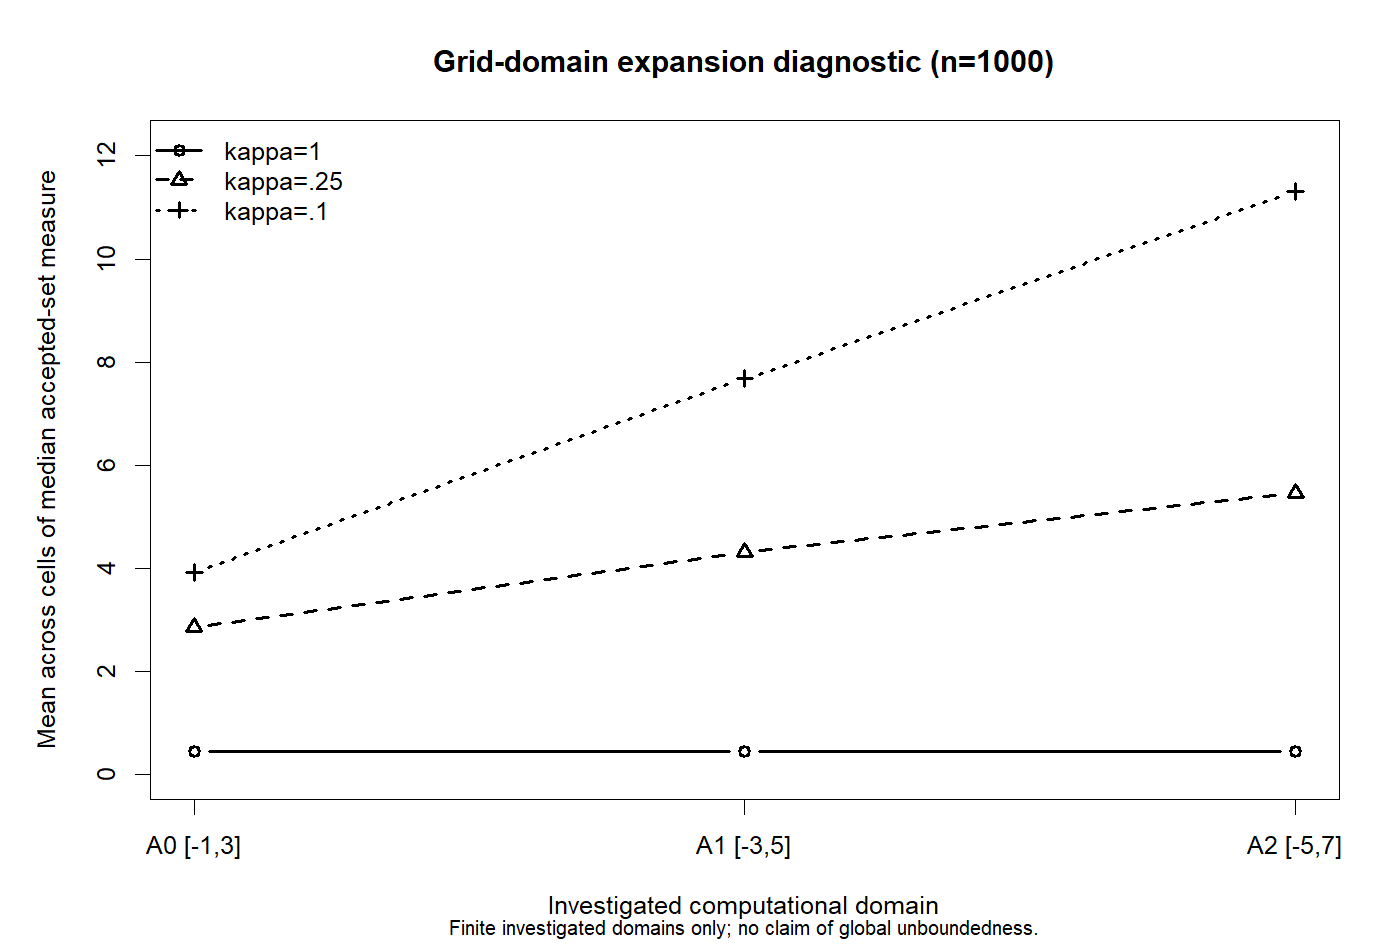
\includegraphics[width=0.72\textwidth]{figures/grid_domain_expansion.png}
  \caption{Sensitivity of the accepted set to expansion of the computational domain}
  \label{fig:grid-domain}
  \begin{figurenotes}[Note]
    Each plotted value is the mean across 15 estimator--quantile cells of the cell-specific median accepted-set measure for the stated $\kappa$ and domain. The investigated domains are $A_0=[-1,3]$, $A_1=[-3,5]$, and $A_2=[-5,7]$. The diagnostic records whether the accepted set stabilizes within these numerical domains; it does not establish global boundedness or unboundedness.
  \end{figurenotes}
\end{figure}

\FloatBarrier

Figure~\ref{fig:appendix_full_domain_acceptance} in Appendix~\ref{app:coverage-forensic-audit} complements these expansion diagnostics by reporting how often all candidates within the primary grid are accepted.
\Needspace{7\baselinedist}
